\documentclass[a4paper]{locconf}
\usepackage{graphicx}
\usepackage[english]{babel}
\usepackage{amsmath}
\usepackage{amsfonts}
\usepackage{amssymb}
\begin{document}
\title{High performance computing for global optimization problems}


\author{K.A. Barkalov, V.P. Gergel}

\address{Lobachevsky State University of Nizhni Novgorod, Gagarin avenue 23, 
Nizhni Novgorod, Russia, 603950}



\begin{abstract}
In the present work, the multiextremal optimization problems and a high-
performance parallel algorithm for solving these ones are considered. The 
investigation of the algorithm scalability has been carried out on the 
problem class, in which the computation costs of the functions depended on 
the iteration point. The algorithm proposed in the present work can utilize 
the CPUs (for solving more complex subproblems) as well as the GPUs (for 
solving the simple subproblems). The results of numerical experiments 
demonstrating the speedup when solving a series of multiextremal constrained 
problems are presented.
\end{abstract}

\section{Introduction}
In the present paper, the constrained multiextremal optimization problems and 
the parallel methods for solving these ones are considered. The fact that the 
global extremum is an integral characteristic of a problem is an important 
feature of the multiextremal problems. Thus, its finding is related to the 
construction of a coverage of the search domain and the computing the 
optimized function values at all points of this coverage. The dimensionality 
affects the difficulty of solving the problems of considered class crucially: 
the computational costs grow with increasing this one exponentially, 
therefore, for solving such problems, the methods are required, which 
generate an essentially nonuniform grid in the search domain, denser in the 
nearness of the global minimum and more sparse far away from this one. In the 
present paper, the results of investigation of the scaling of the parallel 
index global optimization algorithm developed in Lobachevsky State 
University of Nizhni Novgorod \cite{Strongin2000,Strongin2013} and implemented in the Globalizer 
system [NACO] are presented.

Within the framework of the discussed approach, the solving of the 
multidimensional problems is reduced to the solving of a set of the connected 
subproblems of less dimensionality. The corresponding dimensionality 
reduction is based on the use of the evolvents of a unit interval on the real 
axis onto a hypercube. The continuous unambiguous mappings like Peano curves, 
called also the space-filling curves, play the role of such evolvents. 
The nested optimization scheme is one more mechanism used for reducing the 
dimensionality of the problem being solved. The numerical methods allowing 
the efficient utilization of such reduction schemes had been developed 
in details and substantiated in \cite{Strongin2000,Strongin2013}.

In the algorithms developed in the present paper the objective function and constraints are assumed to be Lipschitzian that is typical for many other approaches to the development of the parallel optimization algorithms (see, for example, \cite{Jones,Zilinskas,Evtushenko}). This assumption is natural for many applied problems since the relative variations of the functions generally cannot exceed a certain threshold determined by the bounded energy of changes occurring in the system under study. Also, a standard assumption is that the execution of a single trial (the computing of the values of the objective function and constraints at a point in the search domain) is a time-consuming operation since it 
utilized the results of numerical modeling. 

An assumption on different costs of computing the problem functions subject to 
various components of the vector of parameters is a novel element investigated in the present work. 
It is assumed that it is possible to select the ``difficult'' and ``easy'' parts 
of the functions connected with each other. Then, the solving of the 
``difficult'' part of the problem (for which the execution of the computation-
costly algorithms is required to conduct the trials) can be performed on the 
CPU using an efficient index global optimization algorithm. The ``easy'' part 
of the problem (the execution of which doesn�t require the complex algorithms 
and can be transferred to an accelerator easily) can be solved on a GPU using 
the uniform grid technique. Obviously, in this case a major portion of the trials 
will be performed on the GPUs, and the minor one -- on the CPU. However, 
because of the difference in the difficulties of the subproblems solved on 
different units, a speedup of the algorithm as a whole can be expected. 
The proposed approach has been implemented in Globalizer parallel software 
system for solving the global optimization problem developed in Lobachevsky 
State University of Nizhni Novgorod. 

\section{Problem statement}

Let us consider the $N$-dimensional global optimization problem
\begin{equation}\label{problem}
\varphi(y^\ast)=\min{\left\{\varphi(y): y \in D, \; g_i(y)\leq 0, \; 1 \leq i 
\leq m\right\}}
\end{equation}
with search domain
\begin{equation}\label{D}
D=\left\{y\in R^N: a_j\leq y_j \leq b_j, 1\leq j \leq N \right\}.
%D=\left\{y\in R^N: a_i\leq y_i \leq b_i, 1\leq i \leq N\right\}.
\end{equation}

The objective function $\varphi(y)$ (henceforth denoted by $g_{m+1}(y)$) and
the left-hand sides $g_i(y), \; 1\leq i \leq m$, of the constraints
satisfy the Lipschitz conditions with constants $L_i, \; 1 \leq i \leq
m+1$, respectively, and may be multiextremal. It is assumed that the
functions $g_i(y),\; 1 \leq i \leq m+1$, are defined and computable only in 
the corresponding domains
\[
Q_1=D, \; Q_{i+1}=\left\{y \in Q_i : g_i(y) \leq 0 \right\}, \; 1 \leq i \leq 
m.
\]

These conditions allow for the introduction of a classification of the
points $y \in D$ according to the number $\nu (y)$ of the constraints
computed at this point. 

Thus, a \textit{trial} at a point $y^k \in D$ executed at the $k$-th
iteration of the algorithm will consist in computing the values 
$g_1(y),...,g_\nu(y),$ where the
index $\nu \leq m$ is determined by the conditions
\[
	g_i(y^k )\leq 0, \; 1 \leq i < \nu, \; g_\nu(y^k)>0, \; \nu \leq m.
\]
The occurrence of the first violation of the constraint terminates the
trial. In the case when the point $y^k$ is a feasible one, i.e. when
$y \in Q_{m+1}$, the trial includes the computation of the values of
all the functions of the problems and the index is assumed to be
$\nu=m+1$. The pair of values
\[
\nu=\nu(y^k), \; z^k=g_\nu(y^k)
\]
is a \textit{trial result}.

The parallel index algorithm, which can be applied to solving such problems 
with partially defined functions and which has been implemented in the 
Globalizer system, described in details in \cite{Strongin2013}. The main idea of the algorithm 
consists in the reduction of the initial multidimensional problem to a set of 
the nested subproblems of less dimensionality and the solving of these ones 
in parallel. The dimensionality reduction schemes utilized in the operation 
of the index algorithm are described briefly in the next section.

\section{Dimensionality reduction}

\subsection{Dimensionality reduction using space-filling curves}

The use of Peano curve $y(x)$ 
\begin{equation}
\left\{y\in R^N: -2^{-1}\leq y_i \leq 2^{-1}, 1 \leq i \leq 
N\right\}=\left\{y(x):0\leq x \leq 1 \right\}
\end{equation}
unambiguously mapping the interval of real axis $[0,1]$ onto a $N$-
dimensional cube is the first of the dimensionality reduction methods 
considered.  To implement this method of dimensionality reduction a 
numerically constructed curve (\textit{evolvent}) is used. The evolvent is 
$2^{-m}$ accurate approximation of the theoretical Peano curve in $L_\infty$ 
metric, where $m$ is an evolvent construction parameter. Problems of 
numerical construction of the evolvents and the corresponding theory are 
considered in detail in \cite{Strongin2000}. 

By using this kind of mapping it is possible to reduce the multidimensional 
problem~(\ref{problem}) to a univariate problem
\[
\varphi(y(x^\ast))=\min \left\{\varphi(y(x)): x \in [0,1], \; g_i(y(x))\leq 
0, \; 1 \leq i \leq m\right\}.
\]

The considered dimensionality reduction scheme juxtaposes a
multidimensional problem with lipschitzian functions to a univariate
problem where the corresponding functions satisfy the uniform H{\"o}lder
condition (see \cite{Strongin2000}), i.e.
\[
\left|g_i(y(x'))-g_i (y(x''))\right| \leq H_i \left|x'-x'' \right|^{1/N}, \; 
x',x''\in [0,1], \; 1\leq i \leq m+1.
\]
Here $N$ is the dimensionality of the initial multidimensional problem and
the coefficients $H_i$ are related with the Lipschitz constants $L_i$ of
the initial problem by the inequalities $H_i \leq 2L_i \sqrt{N+3}$.

\subsection{Nested optimization scheme}

Nested optimization scheme is based on relation (see \cite{Strongin2013})
\begin{equation}\label{nested}
\min_{y \in D}{\left\{\varphi(y): \; g_i(y)\leq 0, \; 1 \leq i \leq 
m\right\}}= \min_{u_1\in D_1}\min_{u_2\in D_2}...\min_{u_M\in D_M 
}{\left\{\varphi(y): \; g_i(y)\leq 0, \; 1 \leq i \leq m\right\}},
\end{equation}
which allows replacing the solving of multidimensional problem 
(\ref{problem}) by solving a family of subproblems related to each other 
recursively.
Here we consider vector $y$ as a vector of block variables
\begin{equation}
y=(y_1,y_2,...,y_N)=(u_1,u_2,...,u_M),
\end{equation}
where the $i$-th block variable $u_i$ is a vector of $N_i$ components of 
vector $y$, taken serially i.e. $u_1=(y_1,y_2,...,y_{N_1})$, 
$u_2=(y_{N_1+1},y_{N_1+2},...,y_{N_1+N_2})$,..., $u_M=(y_{N-N_M+1},y_{N-
N_M+2},...,y_{N})$, at that $N_1+N_2+...+N_M=N$. 
The subdomains $D_i, 1 \leq i \leq M$, are projections of initial search 
domain $D$ onto the subspaces corresponding to the variables $u_i, 1 \leq i 
\leq M$. 

In the present study, this scheme has been applied for $M=2$, i.e. only one 
nesting level has been used
\begin{equation}
\min_{y \in D}{\left\{\varphi(y): \; g_i(y)\leq 0, \; 1 \leq i \leq 
m\right\}}= \min_{u_1\in D_1}\min_{u_2\in D_2}{\left\{\varphi(y): \; 
g_i(y)\leq 0, \; 1 \leq i \leq m\right\}}.
\end{equation}

\section{Organization of parallel computing}\label{sec:4}

The organization of the parallel computations with the use of the recursive 
optimization scheme has been considered in details for the shared/distributed 
memory as well as for the accelerators in \cite{Sysoyev,BarkalovLebedev}. However, in these works the 
problems were considered, in which the time of the trial execution didn�t 
depend on the trial point. Here, the problem is considered assuming that in 
the function $\varphi(y_1,...,y_N)$ it is possible to select more difficult 
part $f(y_1,...,y_N)$ (depending on all problem parameters) and a simpler 
part $g(y_s,...,y_N )$ (depending on a part of the parameters only), for 
example, $\varphi(y)= f(y)g(y)$.

The difficult part of the function implies performing some  
computations related to the numerical simulation, which can be performed on the 
CPUs only. The simple part doesn�t imply the complex computations and can be 
computed on an accelerator, for example, GPU. For solving a problem with such 
a structure, one can apply the parallel recursive optimization scheme with 
the use the CPUs at the upper nesting level and the GPUs at the lower one.

\section{Numerical experiments}\label{sec:5}

The recursive scheme of solving the global optimization problems has been 
implemented in the Globzlizer solver developed in Lobachevsky State 
University of Nizhni Novgorod. The global search methods and various 
dimensionality reduction schemes make the algorithmic base for the 
Globalizer. The numerical experiments, the results of which are presented in 
\cite{BarkalovGergelLebedev,BarkalovGergel} demonstrate these methods, at least, are not worse than the well known 
methods applied for similar purposes, and even overcome these ones with 
respect to some parameters. 

Let us conduct the investigation of the scalability of the parallel 
algorithm by solving a series of 100 test problems of the constrained global 
optimization. In work \cite{Gergel2017} the approach has been proposed, which allowed 
generating the constrained global optimization problems with the following 
properties:
\begin{itemize}
	\item one could control the size of the feasible domain $Q_{m+1}$ with 
respect to the whole domain $D$;
	\item the global minimizer of the objective function is known a priori 
taking into account the constraints;
	\item the global minimizer of the objective function without accounting 
for the constraints is out of the feasible domain $Q_{m+1}$  (with the 
purpose of simulating the behavior of the constraints and the objective 
function in the applied constrained optimization problems).
\end{itemize}

In order to simulate the applied problems with various computational 
difficulty, we will use a combination of the function classes of the kind 
\[
\varphi(y_1,...,y_N) = p(y_1,...,y_N)(f(y_1,y_2)+g(y_3,...,y_N)).
\]
Here $f(y_1,y_2)$ is a two-dimensional function from the class described in \cite{Gergel2016}, $g(y_3,...,y_N)$ is a function of the dimensionality $N-2$ from the 
class described in \cite{Sergeyev2015}, and $p(y_1,...,y_N)$ is a second 
order polynomial. The multiplication by $p(y_1,...,y_N)$ excluded the possibility of 
separable search of the minima of the functions $f(y_1,y_2)$ and 
$g(y_3,...,y_N)$. 

The level lines of the two-dimensional subproblems based on the functions 
$f(y_1,y_2)$ and $g(y_3,y_4)$ are shown in figure~1. The feasible domains are highlighted by color. One can see that 
the subproblem (a) has more complex structure as compared to the subproblem 
(b). At the same time, computing the values of the function $f(y_1,y_2)$ is 
more computation-costly than of $g(y_3,y_4)$.

\begin{figure}[ht]
\begin{minipage}[h]{0.5\linewidth}
\center{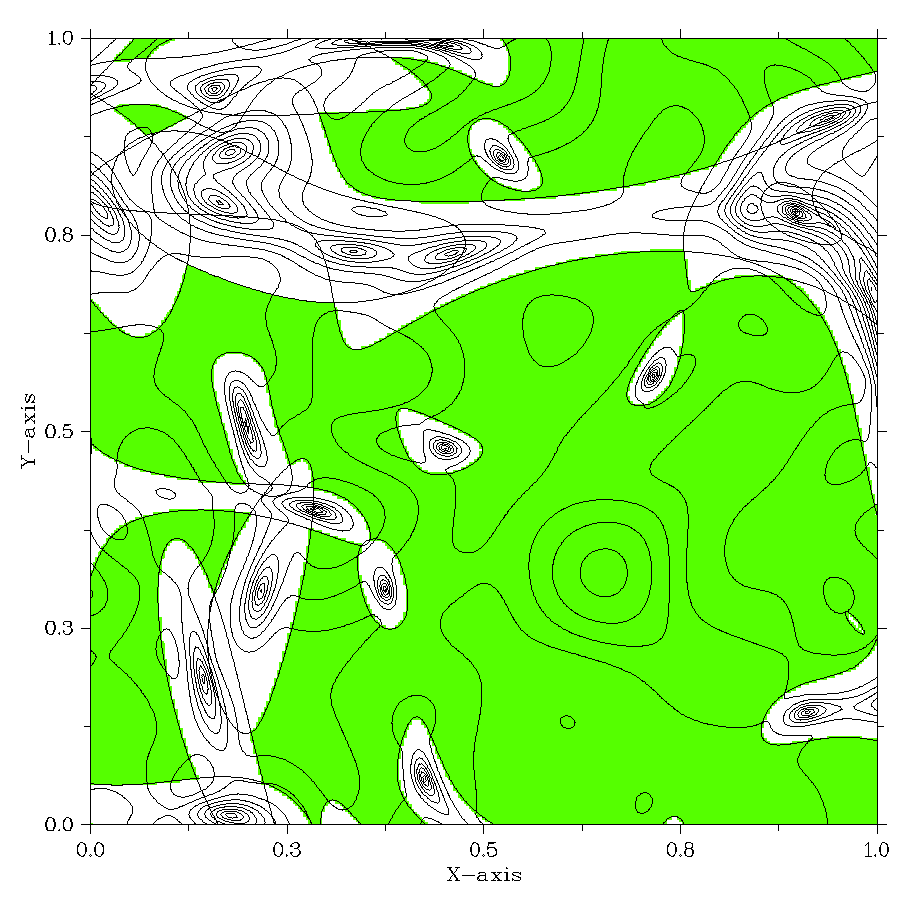
\includegraphics[width=1.0\linewidth]{vag_06.png} \\ (a)}
\end{minipage}
\hfill
\begin{minipage}[h]{0.5\linewidth}
\center{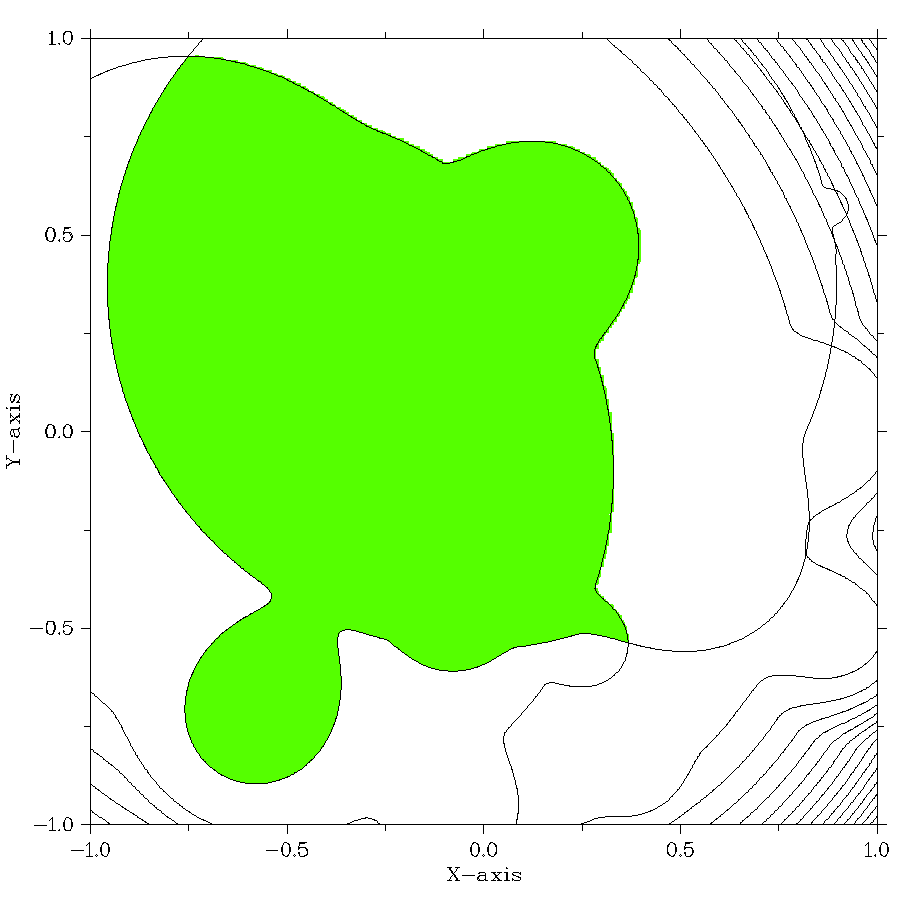
\includegraphics[width=1.0\linewidth]{GKLS_04.png} \\ (b)}
\end{minipage}
\center{{\bf Figure 1.} The level lines of (a) hard and (b) simple 
subproblems}
\end{figure}

The numerical experiments were carried out using two classes of problems 
(\textit{Simple} ans \textit{Hard}) with $N=5$. The problem was considered to 
be solved if the algorithm generates a trial point $y^k$ in $\delta$-vicinity 
of the global minimizer, i.e. $\left\|y^k-y^\ast\right\|\leq\delta$ . The 
size of the vicinity was selected as $\delta=0.01\left\|b-a\right\|$, where 
$a$ and $b$ are the boundaries of the search domain $D$. The maximum 
allowable number of iterations was $K_{max} = 10^6$.

Let us conduct the first experiment by solving the \textit{Simple} and \textit{Hard} problem 
series on a single node employing both available CPUs in full (i. e. $p=16$ 
cores available). In table 1 the averaged time (in seconds) 
required to solve the problems of the series is presented.

\begin{table}[ht]
\center{{\bf Table 1.} Average time for solving the problem on one node}
\begin{center}
\begin{tabular}{cc}
\hline
Problems & Time (sec) \\
\hline
\textit{Hard} & 52  \\
\textit{Simple} & 51 \\
\hline
\end{tabular}
\end{center}
\end{table}

Let us conduct the next experiment employing $p$ nodes each including three 
graphic accelerators. Thus, at $p=32$ total 96 GPU accelerators were employed 
each including 2688 CUDA cores. In table 2, the execution time of the 
algorithm is presented and in table 3 -- the speedup with respect to the run 
on a single node.

\begin{table}[ht]
\center{{\bf Table 2.} Average time for solving the problem on $p$ nodes}
\begin{center}
\begin{tabular}{cccc}
\hline
Problems & $p = 8$ & $p=16$ & $p=32$ \\
\hline
\textit{Hard} & 11.51 & 5.53 & 0.54 \\
\textit{Simple} & 2.04 & 1.50 & 0.47\\
\hline
\end{tabular}
\end{center}
\end{table}

\begin{table}[ht]
\center{{\bf Table 3.} Speedup with respect to one node}
\begin{center}
\begin{tabular}{cccc}
\hline
Problems & $p = 8$ & $p=16$ & $p=32$ \\
\hline
\textit{Hard} & 5 & 9 & 96\\
\textit{Simple} & 25 & 34& 109\\
\hline
\end{tabular}
\end{center}
\end{table}

Computational experiments were carried out on a high-performance cluster of 
Lobachevsky State University of Nizhni Novgorod. The cluster node included 
two Intel Sandy Bridge E5-2660 2.2 GHz CPUs, 64 Gb RAM, and three NVIDIA 
Kepler K20� GPUs (2688 CUDA cores, 6 Gb GDDR5). 
The results of experiments demonstrate that the paralle index algorithm combined with the nested optimization scheme provides a good speedup on the considered problem class. 

%The results of experiments performed on a series of test problems of the constrained global optimization with different time of computing the the problem functions demonstrate the index global optimization algorithm combined with the block recursive scheme for the dimensionality reduction to provide a good speedup on the considered problem class. The directions of further investigations include the expansion of the number of algorithms used for solving the subproblems on the GPUs.

\section*{Acknowledgments}
This study was supported by the Russian Science Foundation, project No 16-11-
10150.

\section*{References}

\medskip

\begin{thebibliography}{9}

\bibitem{Strongin2000}
Strongin, R.G. Global optimization with non-convex constraints. Sequential 
and parallel algorithms. / R.G. Strongin, Ya.D.  Sergeyev --- Dordrecht: 
Kluwer Academic Publishers, 2000. --- 704 p.

\bibitem{Strongin2013}
Strongin, R.G. Parallel computing in global optimization problems / R.G. 
Strongin, V.P. Gergel, V.A. Grishagin, K.A. Barkalov --- Moscow: Publishing 
of the Moscow State University, 2013. --- 280 p. --- (in Russian).

\bibitem{Jones}
Jones, D.R. The DIRECT global optimization algorithm / In: Floudas, C. A., 
Pardalos, P. M. (eds.) The Encyclopedia of Optimization, Second Edition. --- 
Heidelberg: Springer, 2009. --- P. 725--735. 

\bibitem{Zilinskas}
Paulavi\v{c}ius, R. Parallel branch and bound for global optimization with 
combination of Lipschitz bounds / R. Paulavi\v{c}ius, J. \v{Z}ilinskas, A. 
Grothey // Optimization Methods \& Software. --- 2011. --- Vol. 26(3). --- P. 
487--498.

\bibitem{Evtushenko}
Evtushenko, Yu.G. Parallel global optimization of functions of several 
variables / Yu.G. Evtushenko, V.U. Malkova, A.A. Stanevichyus // 
Computational Mathematics and Mathematical Physics. --- 2009. --- Vol. 49 
(2). --- P. 246--260.

\bibitem{Sysoyev}
Sysoyev, A.V. MPI implementation of dimension reduction multilevel scheme for 
parallel solving the global optimization problems / A.V. Sysoyev, K.A. 
Barkalov, V.P. Gergel, I.G. Lebedev // Russian Supercomputing Days: 
Proceedings of the International Scientific Conference. --- Moscow: 
Publishing of the Moscow State University, 2015. --- P. 61--68.

\bibitem{BarkalovLebedev}
Barkalov, K.A. Solving global optimization problems on GPU / K.A. Barkalov, 
I.G. Lebedev // Russian Supercomputing Days: Proceedings of the international 
conference. --- Moscow: Publishing of the Moscow State University, 2016. --- 
P. 640--650.

\bibitem{BarkalovGergel}
Barkalov, K. Parallel global optimization on GPU / K. Barkalov K., V. Gergel 
// Journal of Global Optimization. --- 2016. --- Vol. 66(1). --- P. 3--20.

\bibitem{BarkalovGergelLebedev}
Barkalov, K. Use of Xeon Phi Coprocessor for Solving Global Optimization 
Problems / K. Barkalov, V. Gergel, I. Lebedev //  Lecture Notes in Computer 
Science. --- 2015. --- Vol. 9251. --- P. 307--318.

\bibitem{Gergel2017}
Gergel, V. An Approach for Generating Test Problems of Constrained Global 
Optimization / V. Gergel // Lecture Notes in Computer Science. --- 2017. --- 
Vol. 10556. --- P. 314--319.

\bibitem{Gergel2016}
Gergel, V. Adaptive nested optimization scheme for multidimensional global 
search / V. Gergel, V. Grishagin, A. Gergel // Journal of Global 
Optimization. --- 2016. --- Vol. 66(1). --- P. 35--51.

\bibitem{Sergeyev2015}
Sergeyev, Y.D. (2015) A deterministic global optimization using smooth diagonal auxiliary functions / Y.D. Sergeyev, D.E. Kvasov // Communications in Nonlinear Science and Numerical Simulation. --- 2015. --- Vol. 21 (1-3). --- P. 99--111.

\end{thebibliography}

\end{document}


